% ============================================================
%   EPSS-TPG abstract model architecture (two-column figure)
% ============================================================
%
% Single horizontal-flow overview, sized for a paper's wide
% (full-width) figure in a two-column layout. The page is sized
% to the figure's natural bounding box so
%   
\includegraphics[width=\linewidth]{model_architecture_abstract}
% scales to the column width without extra white space.
%
% Companion: model_architecture.tex (the detailed A2 reference).
%
% Compile:
%   pdflatex -interaction=nonstopmode model_architecture_abstract.tex
% ============================================================

\documentclass[10pt]{article}

% Page sized close to the figure bounding box.
\usepackage[paperwidth=300mm, paperheight=115mm, margin=4mm]{geometry}
\usepackage{tikz}
\usepackage{amsmath}
\usepackage{amssymb}
\pagestyle{empty}

\usetikzlibrary{positioning, arrows.meta, calc, fit, backgrounds}

% Colour palette (printer-friendly, distinguishable in grayscale).
\definecolor{cText}{RGB}{236,244,255}      % input  (light blue)
\definecolor{cTPG}{RGB}{223,239,223}       % TPG    (light green)
\definecolor{cEmb}{RGB}{240,228,247}       % embed  (light purple)
\definecolor{cGNN}{RGB}{217,237,237}       % GNN    (light teal)
\definecolor{cTab}{RGB}{255,222,222}       % tab    (light pink)
\definecolor{cHead}{RGB}{229,229,229}      % head   (light grey)
\definecolor{cOut}{RGB}{255,247,210}       % output (light yellow)
\definecolor{accent}{RGB}{20,70,140}

\tikzset{
    box/.style={
        rectangle, rounded corners=2pt, draw=black!55,
        line width=0.45pt, inner sep=4pt,
        align=center, font=\small,
        minimum height=15mm, minimum width=24mm,
    },
    boxsmall/.style={
        rectangle, rounded corners=2pt, draw=black!55,
        line width=0.45pt, inner sep=3pt,
        align=center, font=\scriptsize,
        minimum height=11mm, minimum width=24mm,
    },
    flow/.style={
        -{Stealth[length=2.5mm]}, line width=0.55pt, draw=black!75
    },
    branch/.style={
        -{Stealth[length=2mm]}, line width=0.5pt, draw=black!70
    },
    bandlabel/.style={font=\sffamily\bfseries\small, text=accent, align=center},
    edgelab/.style={font=\scriptsize, text=black!55, inner sep=1pt},
}

\begin{document}

\noindent
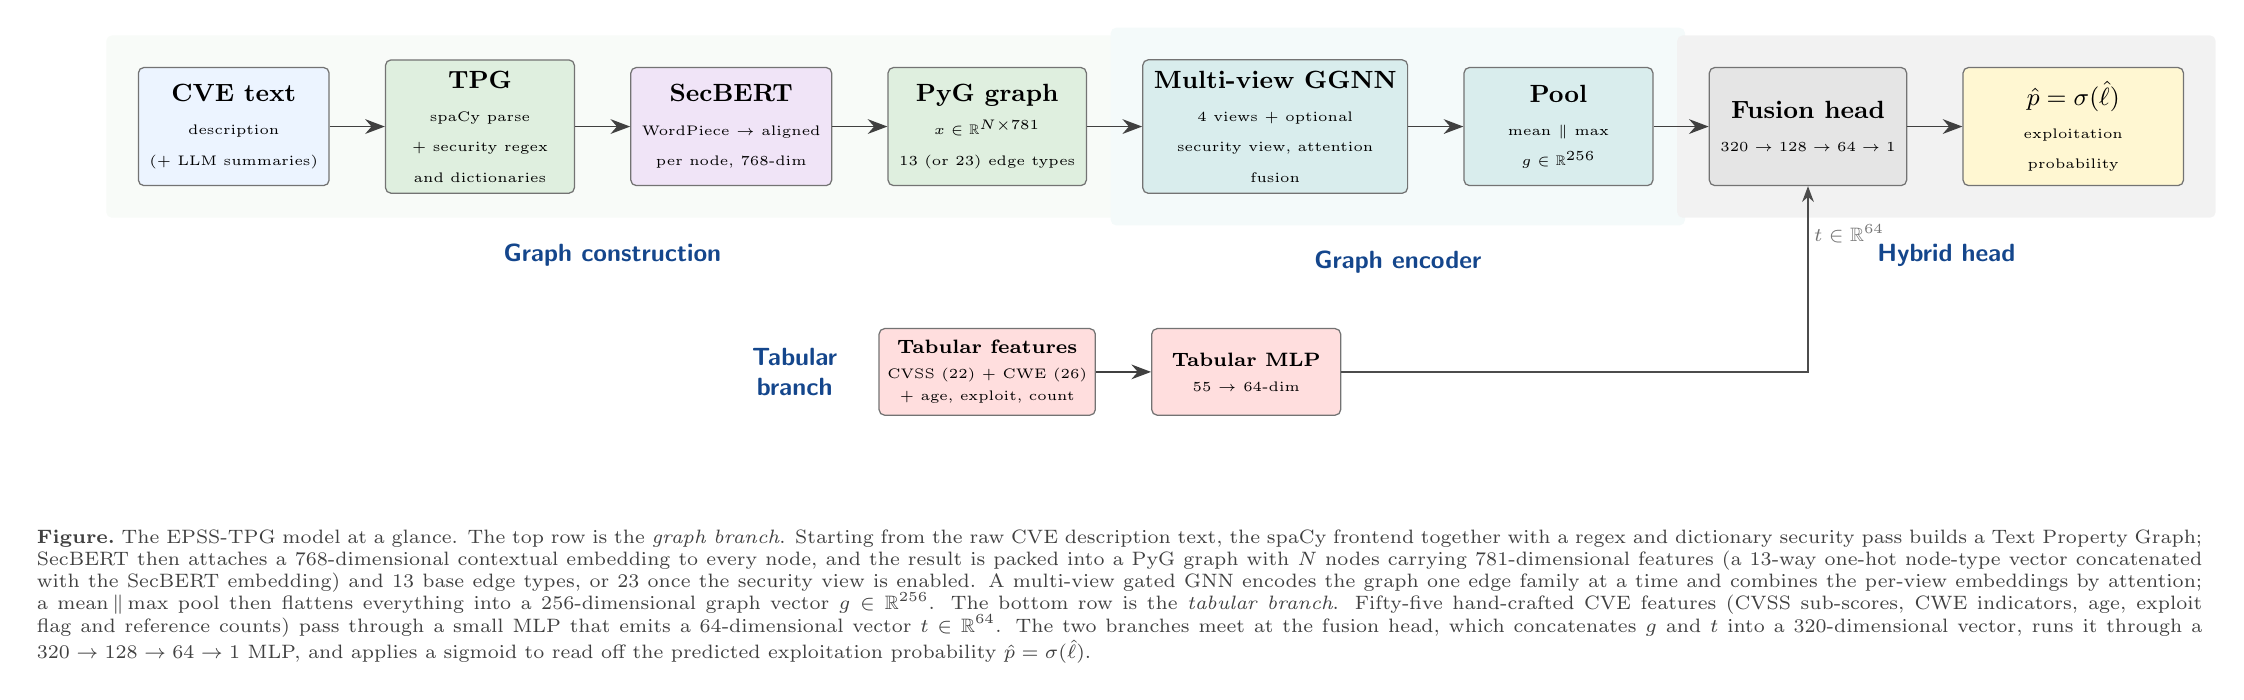
\begin{tikzpicture}[node distance=8mm and 7mm]

% ============================================================
%  Row 1: graph branch (left-to-right pipeline)
% ============================================================
% Box content is kept tight: title in bold, one or two lines of small
% supporting text per box, with key dimensions stated inside the box
% so arrows do not need captions.

\node[box, fill=cText] (text) {
    \textbf{CVE text}\\[1pt]
    {\tiny description}\\
    {\tiny (+ LLM summaries)}
};

\node[box, fill=cTPG, right=of text] (tpg) {
    \textbf{TPG}\\[1pt]
    {\tiny spaCy parse}\\
    {\tiny + security regex}\\
    {\tiny and dictionaries}
};

\node[box, fill=cEmb, right=of tpg] (sbert) {
    \textbf{SecBERT}\\[1pt]
    {\tiny WordPiece $\to$ aligned}\\
    {\tiny per node, 768-dim}
};

\node[box, fill=cTPG, right=of sbert] (pyg) {
    \textbf{PyG graph}\\[1pt]
    {\tiny $x \in \mathbb{R}^{N \times 781}$}\\
    {\tiny 13 (or 23) edge types}
};

\node[box, fill=cGNN, right=of pyg, minimum width=30mm] (mv) {
    \textbf{Multi-view GGNN}\\[1pt]
    {\tiny 4 views + optional}\\
    {\tiny security view, attention}\\
    {\tiny fusion}
};

\node[box, fill=cGNN, right=of mv] (pool) {
    \textbf{Pool}\\[1pt]
    {\tiny mean $\Vert$ max}\\
    {\tiny $g \in \mathbb{R}^{256}$}
};

\node[box, fill=cHead, right=of pool] (head) {
    \textbf{Fusion head}\\[1pt]
    {\tiny $320 \to 128 \to 64 \to 1$}
};

\node[box, fill=cOut, right=of head, minimum width=28mm] (out) {
    $\hat p = \sigma(\hat\ell)$\\[1pt]
    {\tiny exploitation}\\
    {\tiny probability}
};

% Flow arrows along the top row. Clean lines, no captions.
\draw[flow] (text)  -- (tpg);
\draw[flow] (tpg)   -- (sbert);
\draw[flow] (sbert) -- (pyg);
\draw[flow] (pyg)   -- (mv);
\draw[flow] (mv)    -- (pool);
\draw[flow] (pool)  -- (head);
\draw[flow] (head)  -- (out);

% ============================================================
%  Row 2: tabular branch (parallel, joins at fusion head)
% ============================================================
% Place the two tabular boxes underneath the middle of the top row.
% The branch joins the fusion head from below.

\node[boxsmall, fill=cTab, below=18mm of pyg] (tab) {
    \textbf{Tabular features}\\[1pt]
    {\tiny CVSS (22) + CWE (26)}\\
    {\tiny + age, exploit, count}
};

\node[boxsmall, fill=cTab, right=of tab] (tabmlp) {
    \textbf{Tabular MLP}\\[1pt]
    {\tiny 55 $\to$ 64-dim}
};

\draw[flow] (tab) -- (tabmlp);

% Tabular path: right, then up into the head from below.
% Anchor the elbow so it never sits on top of any box.
\coordinate (elbow) at ($(head.south) + (0,-12mm)$);
\draw[branch] (tabmlp.east) -| (elbow) -- (head.south)
    node[edgelab, midway, right=1pt] {$t \in \mathbb{R}^{64}$};

% Single tiny label on the top-row arrow that crosses the elbow
% area is unnecessary; the Pool box already shows g and the Fusion
% box already shows the input dim implicitly. Keep the figure free of
% inline arrow captions.

% ============================================================
%  Group bands behind the boxes (semantic colour grouping)
% ============================================================
\begin{scope}[on background layer]
    \node[fit=(text)(pyg), inner sep=4mm,
          fill=cTPG!22, rounded corners=2pt] (bandA) {};
    \node[fit=(mv)(pool), inner sep=4mm,
          fill=cGNN!28, rounded corners=2pt] (bandB) {};
    \node[fit=(head)(out), inner sep=4mm,
          fill=cHead!50, rounded corners=2pt] (bandC) {};
\end{scope}

% Band titles. Placed below the bands so they cannot clash with
% any arrow caption above.
\node[bandlabel, below=2mm of bandA.south] {Graph construction};
\node[bandlabel, below=2mm of bandB.south] {Graph encoder};
\node[bandlabel, below=2mm of bandC.south] {Hybrid head};

% Tabular branch label, sitting at the left of the tabular row.
\node[bandlabel, left=4mm of tab.west] {Tabular\\branch};

% ============================================================
%   Caption (below the figure). Kept inside the standalone
%   bounding box so the figure is self-contained when viewed
%   on its own. When the figure is included in a paper via
%   \includegraphics{}, prefer the suggested \caption{...}
%   block reproduced as a comment at the end of this file.
% ============================================================
\node[font=\scriptsize, text=black!75, text width=275mm,
      align=justify, anchor=north] (cap) at (11.25, -5.0) {%
    \textbf{Figure.}\ The EPSS-TPG model at a glance. The top
    row is the \emph{graph branch}. Starting from the raw
    CVE description text, the spaCy frontend together with
    a regex and dictionary security pass builds a Text
    Property Graph; SecBERT then attaches a 768-dimensional
    contextual embedding to every node, and the result is
    packed into a PyG graph with $N$ nodes carrying
    781-dimensional features (a 13-way one-hot node-type
    vector concatenated with the SecBERT embedding) and 13
    base edge types, or 23 once the security view is
    enabled. A multi-view gated GNN encodes the graph one
    edge family at a time and combines the per-view
    embeddings by attention; a mean$\,\Vert\,$max pool then
    flattens everything into a 256-dimensional graph vector
    $g \in \mathbb{R}^{256}$. The bottom row is the
    \emph{tabular branch}. Fifty-five hand-crafted CVE
    features (CVSS sub-scores, CWE indicators, age, exploit
    flag and reference counts) pass through a small MLP that
    emits a 64-dimensional vector $t \in \mathbb{R}^{64}$.
    The two branches meet at the fusion head, which
    concatenates $g$ and $t$ into a 320-dimensional vector,
    runs it through a $320 \to 128 \to 64 \to 1$ MLP, and
    applies a sigmoid to read off the predicted exploitation
    probability $\hat p = \sigma(\hat\ell)$.
};

\end{tikzpicture}

\end{document}

% ============================================================
%   Suggested LaTeX caption for paper integration
% ============================================================
%
% Copy this into a \begin{figure*}...\end{figure*} block:
%
% \begin{figure*}[t]
%   \centering
%   
\includegraphics[width=\linewidth]{model_architecture_abstract}
%   \caption{The EPSS-TPG model at a glance. The top row is
%   the graph branch: starting from the raw CVE description
%   text, the spaCy frontend together with a regex and
%   dictionary security pass builds a Text Property Graph,
%   SecBERT attaches a 768-dimensional contextual embedding
%   to every node, and the result is packed into a PyG
%   graph with $N$ nodes carrying 781-dimensional features
%   and 13 (or 23, with the security view enabled) edge
%   types. A multi-view gated GNN encodes the graph one
%   edge family at a time and combines the per-view
%   embeddings by attention; a mean$\,\Vert\,$max pool
%   produces a 256-dimensional graph vector
%   $g \in \mathbb{R}^{256}$. The bottom row is the tabular
%   branch: fifty-five hand-crafted CVE features pass
%   through a small MLP that emits a 64-dimensional vector
%   $t \in \mathbb{R}^{64}$. The two branches meet at the
%   fusion head, which concatenates $g$ and $t$ into a
%   320-dimensional vector, runs it through a
%   $320 \to 128 \to 64 \to 1$ MLP, and applies a sigmoid to
%   read off the predicted exploitation probability
%   $\hat p = \sigma(\hat\ell)$.}
%   \label{fig:model-architecture-abstract}
% \end{figure*}
%
% ============================================================
